\documentclass[namecite, fleqn]{goose-article}

\title{%
    Elasto-plastic continuum model
    based on a manifold of quadratic potentials
}

\author{Tom W.J.\ de Geus}

\hypersetup{pdfauthor={T.W.J. de Geus}}

\newcommand\leftstar[1]{\hspace*{-.3em}~^\star\!#1}

\newcommand\T[1]{\underline{\bm{{#1}}}}

\newcommand\TT[1]{\underline{\mathbb{{#1}}}}

\begin{document}

\maketitle

\begin{abstract}
\noindent
A microscopic continuum model of plasticity in amorphous solids is proposed.
This model uses a strain energy with multiple minima to capture the effect of plasticity.
This model was used for the first time in \citet{DeGeus2018}
and was partly inspired on the work of \citet{Jagla2017}.

\keywords{elasto-plasticity; linear elasticity}
\end{abstract}

\setcounter{tocdepth}{3}
\tableofcontents

\vfill\newpage
\section{General model}

The model is constructed such that it behaves linear elastically in the volumetric stress response.
The same holds for the deviatoric stress response, whereby plasticity is modelled
such that the material starts flowing once a critical strain is reached.
After a period of flow, the deviatoric stress response is again linear elastic.

Below underlined bold symbols $\T{A}$ are tensors, while normal symbols $A$ are scalars.
Strains are denoted by $\varepsilon$ while stresses are denoted by $\sigma$.
Subscripts $(.)_\mathrm{m}$ and $(.)_\mathrm{d}$ are used to indicate the
volumetric and deviatoric part of the strains and stress.
Furthermore, the elastic moduli and the equivalent stress and strain are defined such
(i) that the model is equivalent regardless of the number of dimensions, $d$;
(ii) for simple shear the equivalent deviatoric strain is equal to $\varepsilon_\mathrm{xy}$;
(iii) $\sigma_\mathrm{xy} = G \varepsilon_\mathrm{xy}$, with $G$ the shear modulus.
To retrieve another common definition for linear elasticity in $d = 3$,
one simply has to rescale the parameters.
See the appendices for the full nomenclature, including the parameter transformation.

The model is based on a strain energy $W$ that is composed of two parts,
a hydrostatic (or volumetric) part $U$ related to the hydrostatic strain $\varepsilon_\mathrm{m}$,
and a deviatoric (or shear) part $V$ related to the
equivalent shear strain $\varepsilon_\mathrm{d}$, i.e.
\begin{equation}
    W(\T{\varepsilon}) = U(\varepsilon_\mathrm{m}) + V(\varepsilon_\mathrm{d})
\end{equation}
The stress response $\T{\sigma}$ is the derivative of this energy with respect
to the strain tensor $\T{\varepsilon}$.
Before specialising $U$ and $V$ we can already say that
\begin{equation}
    \label{eq:dU-dV:elas}
    \T{\sigma}
    =
    \frac{\partial W}{\partial \T{\varepsilon}}
    =
    \frac{\partial U}{\partial \varepsilon_\mathrm{m}} \;
    \frac{\partial \varepsilon_\mathrm{m}}{\partial \T{\varepsilon}}
    +
    \frac{\partial V}{\partial \varepsilon_\mathrm{d}} \;
    \frac{\partial \varepsilon_\mathrm{d}}{\partial \T{\varepsilon}}
    =
    \frac{\partial U}{\partial \varepsilon_\mathrm{m}} \;
    \frac{1}{d} \T{I}
    +
    \frac{\partial V}{\partial \varepsilon_\mathrm{d}} \;
    \frac{1}{2} \frac{\T{\varepsilon}_\mathrm{d}}{\varepsilon_\mathrm{d}}
    =
    \frac{1}{d} \;
    \frac{\partial U}{\partial \varepsilon_\mathrm{m}} \;
    \T{I}
    +
    \frac{1}{2}
    \frac{\partial V}{\partial \varepsilon_\mathrm{d}} \;
    \T{N}_\mathrm{d}
\end{equation}
Below, both $U(\varepsilon_\mathrm{m})$ and $V(\varepsilon_\mathrm{d})$
will be defined by slowly increasing complexity, departing from linear elasticity.

\subsection{Linear elasticity}

We start simple by considering linear elasticity.
In this case the volumetric strain energy $U$ and the shear strain energy $V$ read
\begin{align}
    \label{eq:W:elas}
    U (\varepsilon_\mathrm{m})
    &= \frac{d}{2} \, K \, \varepsilon_\mathrm{m}^2
    \\
    \label{eq:V:elas}
    V (\varepsilon_\mathrm{d})
    &= G \, \varepsilon_\mathrm{d}^2
\end{align}
The two potentials are plotted in \cref{fig:U-V:elas}
(only $\varepsilon_\mathrm{d} \geq 0$ is shown, as it is by definition non-negative).
It is trivial to obtain that
\begin{align}
    \frac{\partial U}{\partial \varepsilon_\mathrm{m}}
    &= d \, K \, \varepsilon_\mathrm{m}
    \\
    \frac{\partial V}{\partial \varepsilon_\mathrm{d}}
    &= 2 \, G \, \varepsilon_\mathrm{d}
\end{align}
(plotted in \cref{fig:dU-dV:elas}).
From which we obtain the following expression for the stress
\begin{equation}
    \label{eq:sig-elas}
    \T{\sigma} ( \T{\varepsilon} )
    =
    K \, \varepsilon_\mathrm{m} \, \T{I}
    +
    G \, \varepsilon_\mathrm{d} \, \T{N}_\mathrm{d}
    =
    K \, \varepsilon_\mathrm{m} \, \T{I}
    +
    G \, \T{\varepsilon}_\mathrm{d}
\end{equation}
where the direction of shear is contained in
\begin{equation}
    \T{N}_\mathrm{d} \equiv \frac{\T{\varepsilon}_\mathrm{d}}{\varepsilon_\mathrm{d}}
\end{equation}
Note that
\begin{equation}
    \sqrt{\tfrac{1}{2} \T{N}_\mathrm{d} : \T{N}_\mathrm{d}} = 1,
    \qquad
    \frac{
        \partial \varepsilon_\mathrm{d}
    }{
        \partial \T{\varepsilon}_\mathrm{d}
    }
    = \tfrac{1}{2} \T{N}_\mathrm{d}
\end{equation}
(see \cref{sec:nomenclature:derivatives}).

\begin{figure}[htp]
    \centering
    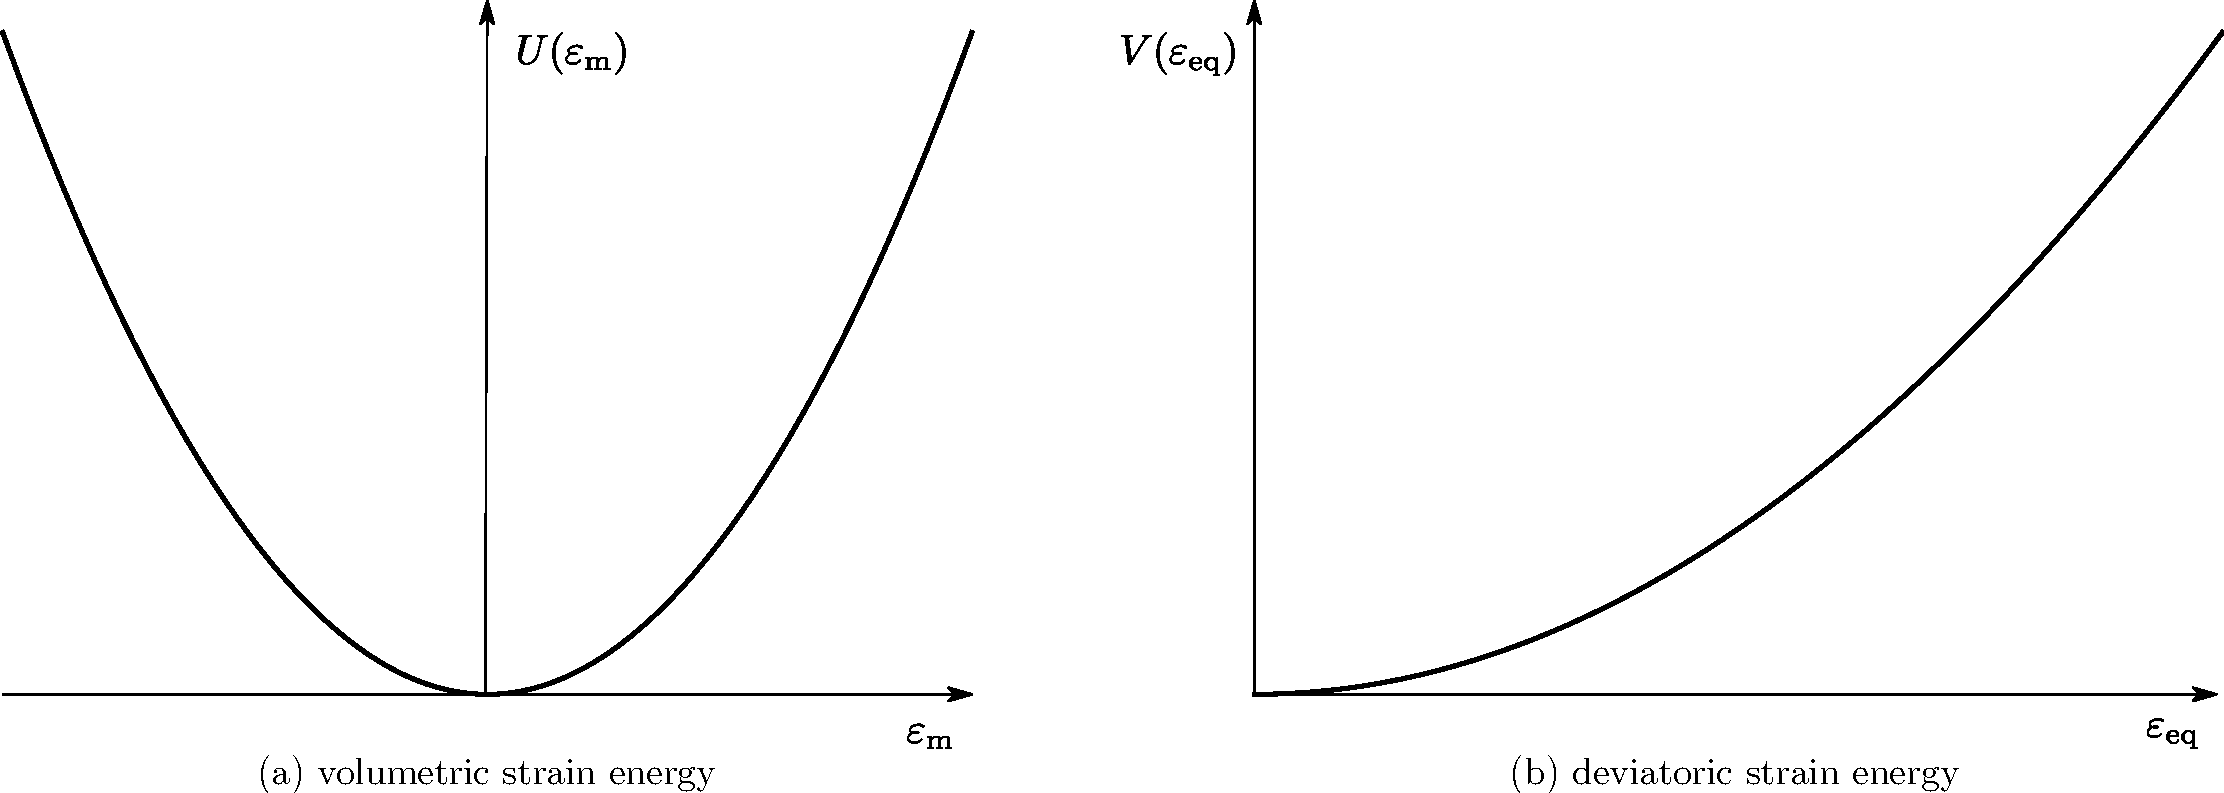
\includegraphics[width=1.\textwidth]{figures/potential_U-V_elas}
    \caption{
        Strain energy
        $W(\T{\varepsilon}) = U(\varepsilon_\mathrm{m}) + V(\varepsilon_\mathrm{d})$
        for linear elasticity.}
    \label{fig:U-V:elas}
\end{figure}

\begin{figure}[htp]
    \centering
    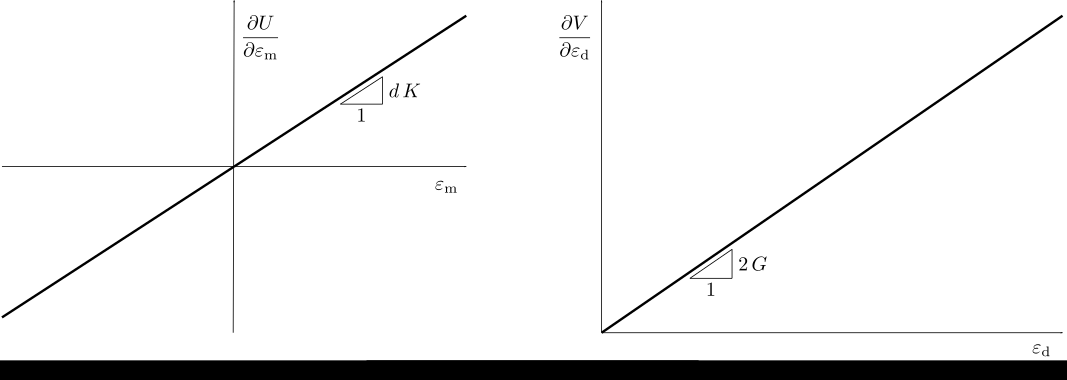
\includegraphics[width=1.\textwidth]{figures/potential_dU-dV_elas}
    \caption{
        Derivative of the hydrostatic strain energy $U$ and the deviatoric strain energy $V$
        w.r.t.\ respectively the hydrostatic strain $\varepsilon_\mathrm{m}$ and
        the equivalent shear strain $\varepsilon_\mathrm{d}$.}
    \label{fig:dU-dV:elas}
\end{figure}

\subsection{Plastic potential -- Parabolic potential with multiple minima}

The model is now extended to account for plasticity.
The model is defined such that the material responds volumetrically purely elastic,
while in shear the model is governed by multiple minima.
These minima have the effect that when the material reaches a certain yield stress,
it jumps to the next minimum.
Around this minimum the elasticity is always the same.
When loading is continued the the material again jumps to a new minimum
when the next yield stress is reached.
The magnitude of the jumps and of the yield stress are thereby related.

As described, the volumetric behaviour is simply elastic; whereby the potential is given by
\cref{eq:W:elas} and is plotted in \cref{fig:U-V:elas}(a).
To attain the desired behaviour in shear, the equivalent shear strain space is divided in a
finite number of yield strains $\varepsilon_\mathrm{y}^{(0)},
\varepsilon_\mathrm{y}^{(1)}, \varepsilon_\mathrm{y}^{(2)}, ...$.
A parabolic potential is then defined between each pair
($[ \varepsilon_\mathrm{y}^{(0)}, \varepsilon_\mathrm{y}^{(1)} )$,
 $[ \varepsilon_\mathrm{y}^{(1)}, \varepsilon_\mathrm{y}^{(2)} )$, ...).

The shear strain energy is then composed of a manifold of quadratic contributions
\begin{equation}
    \label{eq:V-plas}
    V \big(
        \varepsilon_\mathrm{y}^{(i)} \leq \varepsilon_\mathrm{d} < \varepsilon_\mathrm{y}^{(i+1)}
    \big)
    =
    V^{(i)}
    =
    G \, \bigg[\,
        \Big[\, \varepsilon_\mathrm{d} - \varepsilon_\mathrm{min}^{(i)} \,\Big]^2
        -
        \Big[\, \Delta \varepsilon_\mathrm{y}^{(i)} \,\Big]^2
    \,\bigg]
\end{equation}
where the mean of $\varepsilon_\mathrm{y}^{(i)}$ and $\varepsilon_\mathrm{y}^{(i+1)}$ is
\begin{equation}
    \varepsilon_\mathrm{min}^{(i)}
    =
    \tfrac{1}{2} \Big[\, \varepsilon_\mathrm{y}^{(i+1)} + \varepsilon_\mathrm{y}^{(i)} \,\Big]
\end{equation}
which is also the equivalent shear strain at which the shear strain energy reaches its minimum.
From this minimum, the distance to $\varepsilon_\mathrm{y}^{(i)}$ and
$\varepsilon_\mathrm{y}^{(i+1)}$ is
\begin{equation}
    \Delta \varepsilon_\mathrm{y}^{(i)}
    =
    \tfrac{1}{2} \Big[\, \varepsilon_\mathrm{y}^{(i+1)} - \varepsilon_\mathrm{y}^{(i)} \,\Big]
\end{equation}
The resulting shear strain energy is plotted in \cref{fig:V:plas}(a).

The stress response is obtained from
\begin{equation}
    \label{eq:dV-plas}
    \frac{\partial V^{(i)}}{\partial \varepsilon_\mathrm{d}}
    =
    2 \, G \, \Big[\, \varepsilon_\mathrm{d} - \varepsilon_\mathrm{min}^{(i)} \,\Big]
\end{equation}
(see \cref{fig:dV:plas}(a)).
From which it can be observed that in elasticity the behaviour is identical to above
(cf.~\cref{eq:dU-dV:elas}).
For the case that $\varepsilon_\mathrm{y}^{(0)} = - \varepsilon_\mathrm{y}^{(1)}$ the
responses are even identical until initial yield stress is reached.
For completeness, the stress reads
\begin{equation}
    \T{\sigma} ( \T{\varepsilon} )
    =
    K \, \varepsilon_\mathrm{m} \, \T{I}
    +
    G \, \Big[\, \varepsilon_\mathrm{d} - \varepsilon_\mathrm{min}^{(i)} \,\Big] \;
    \T{N}_\mathrm{d}
    \qquad
    \mathrm{for}
    \;
    \varepsilon_\mathrm{y}^{(i)} \leq \varepsilon_\mathrm{d} < \varepsilon_\mathrm{y}^{(i+1)}
\end{equation}
whereby one has to assume that when $\varepsilon_\mathrm{d} = 0$ also
$\T{\sigma}_\mathrm{d} = \T{0}$ in order to avoid zero division.
The response is plotted in \cref{fig:dV:plas}(a),
from which it is observed that it exhibits stress jumps between different parabola in the potential,
because of the discontinuity in the second derivative of the elastic potential.
This can be remedied, such as in the model presented below.

\subsection{Plastic potential -- Smooth parabolic potential with multiple minima}

The remedy the discontinuity in the second derivative of the potential, it is smoothed as follows:
\begin{equation}
    \label{eq:V-plas-smooth}
    V \big(
        \varepsilon_\mathrm{y}^{(i)} \leq \varepsilon_\mathrm{d} < \varepsilon_\mathrm{y}^{(i+1)}
    \big)
    =
    V^{(i)}
    =
    - 2 \, G \,
    \left[ \frac{\Delta \varepsilon_\mathrm{y}^{(i)}}{\pi} \right]^2
    \left[
        1 + \cos \left(
          \frac{ \pi }{ \Delta \varepsilon_\mathrm{y}^{(i)} }
          \Big[\, \varepsilon_\mathrm{d} - \varepsilon_\mathrm{min}^{(i)} \,\Big]
        \right)
    \right]
\end{equation}
which is plotted in \cref{fig:V:plas}(b).
In this case the stress is obtained from
\begin{equation}
    \label{eq:dV-plas-smooth}
    \frac{\partial V^{(i)}}{\partial \varepsilon_\mathrm{d}}
    =
    2 \, G \,
    \left[ \frac{\Delta \varepsilon_\mathrm{y}^{(i)}}{\pi} \right]
    \sin \left(
        \frac{ \pi }{ \Delta \varepsilon_\mathrm{y}^{(i)} }
        \Big[\, \varepsilon_\mathrm{d} - \varepsilon_\mathrm{min}^{(i)} \,\Big]
    \right)
\end{equation}
(see \cref{fig:dV:plas}(b)).
Which is to the first order equal to linear elasticity around its minimum
$\varepsilon_\mathrm{min}^{(i)}$.
Indeed, the first order Taylor series of \cref{eq:dV-plas-smooth} around
$\varepsilon_\mathrm{d} = \varepsilon_\mathrm{min}^{(i)}$,
\begin{equation}
    \frac{\partial V^{(i)}}{\partial \varepsilon_\mathrm{d}}
    \approx
    2 \, G \, \Big[\, \varepsilon_\mathrm{d} - \varepsilon_\mathrm{min}^{(i)} \,\Big]
\end{equation}
is identical to \cref{eq:dV-plas}.

For completeness, also in case the expression for the entire stress tensor
\begin{equation}
    \T{\sigma} ( \T{\varepsilon} )
    =
    K \, \varepsilon_\mathrm{m} \, \T{I}
    +
    G \,
    \left[ \frac{\Delta \varepsilon_\mathrm{y}^{(i)}}{\pi} \right]
    \sin \left(
        \frac{ \pi }{ \Delta \varepsilon_\mathrm{y}^{(i)} }
        \Big[\, \varepsilon_\mathrm{d} - \varepsilon_\mathrm{min}^{(i)} \,\Big]
    \right)
    \T{N}_\mathrm{d}
    \qquad
    \mathrm{for}
    \;
    \varepsilon_\mathrm{y}^{(i)} \leq \varepsilon_\mathrm{d} < \varepsilon_\mathrm{y}^{(i+1)}
\end{equation}
whereby, again, one has to assume that when $\varepsilon_\mathrm{d} = 0$ also
$\T{\sigma}_\mathrm{d} = \T{0}$ in order to avoid zero division.

\begin{figure}[htp]
    \centering
    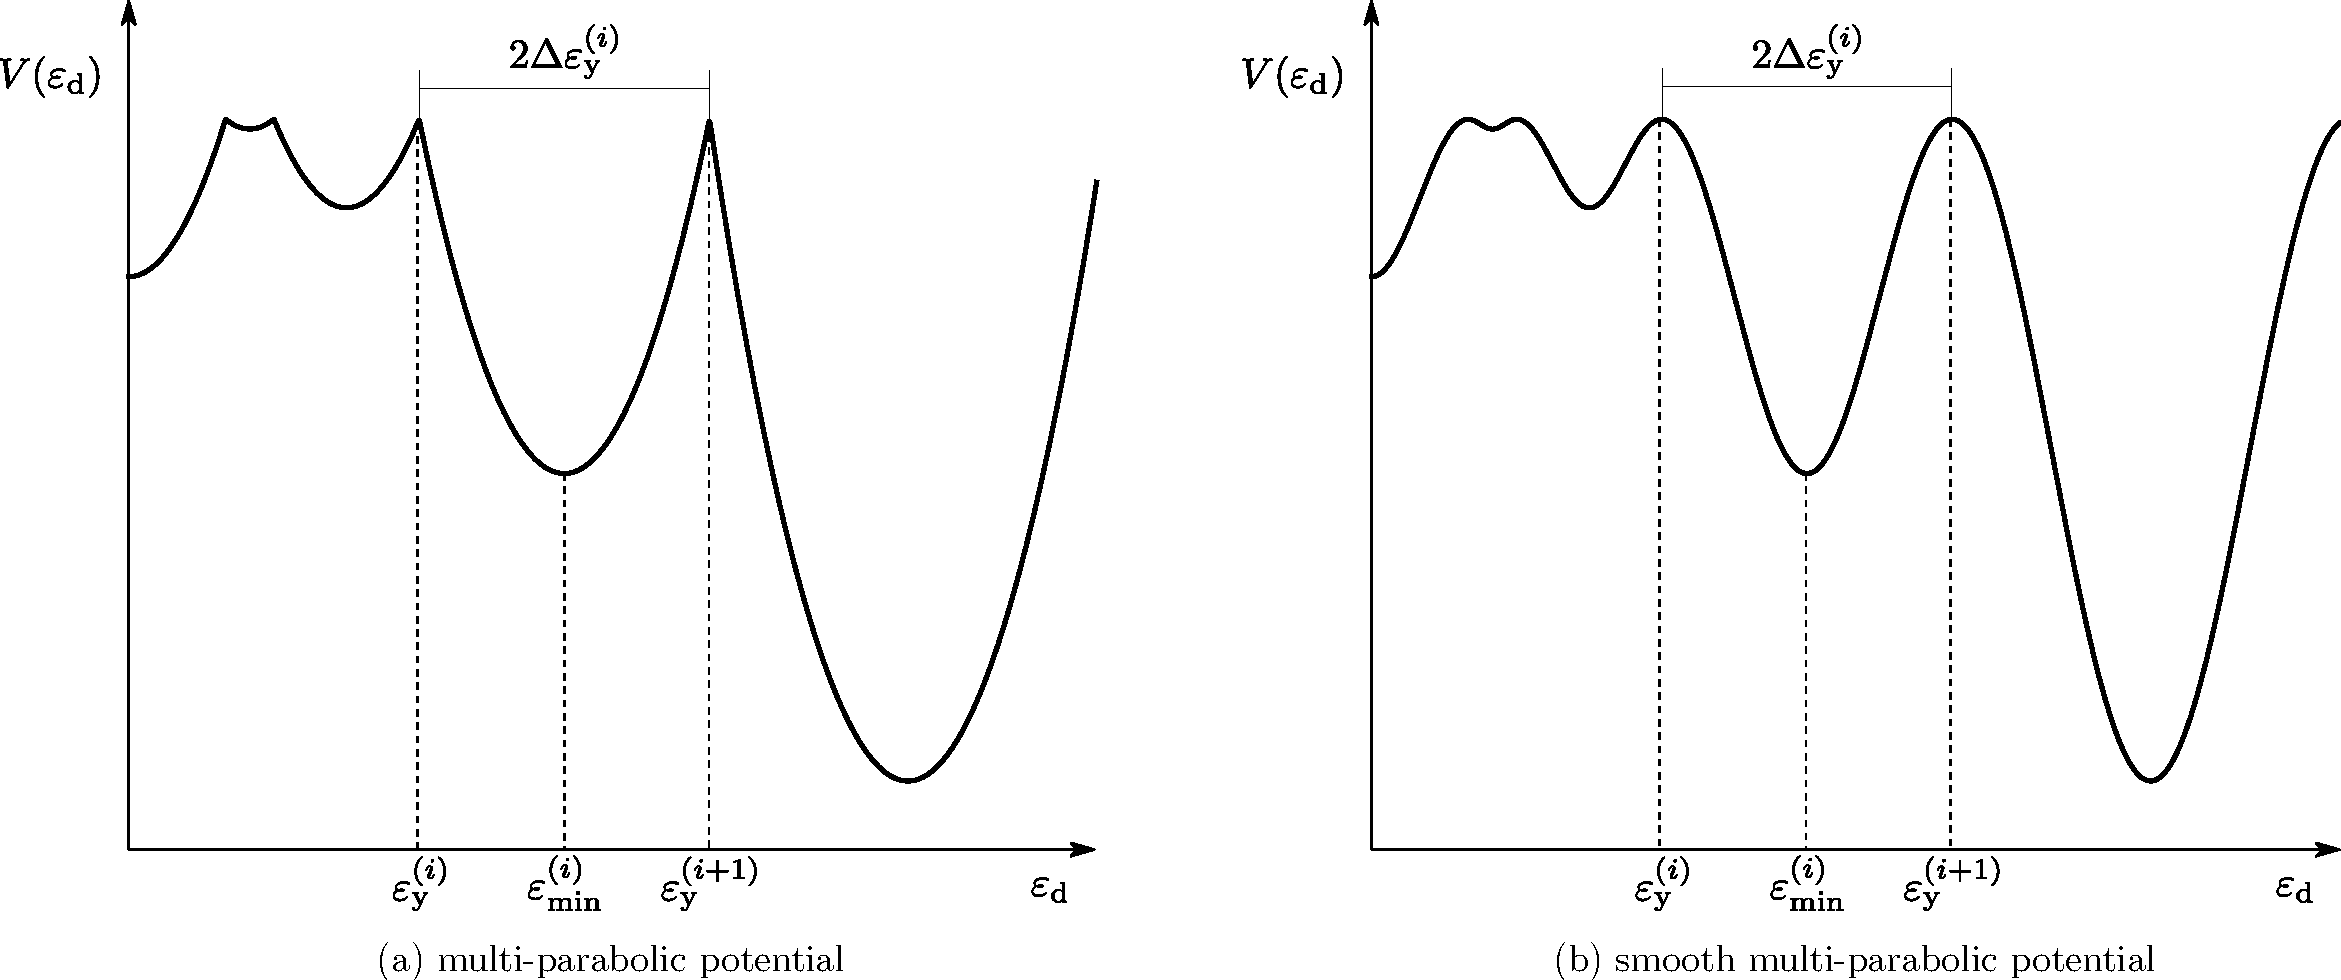
\includegraphics[width=1.\textwidth]{figures/potential_V-plas}
    \caption{
        The multi-minima shear strain energy, $V ( \varepsilon_\mathrm{d} )$,
        that models the effect of plasticity.
    The multi-parabolic shear strain energy is shown in (a),
    while its smoothed equivalent is shown in (b).}
    \label{fig:V:plas}
\end{figure}

\begin{figure}[htp]
    \centering
    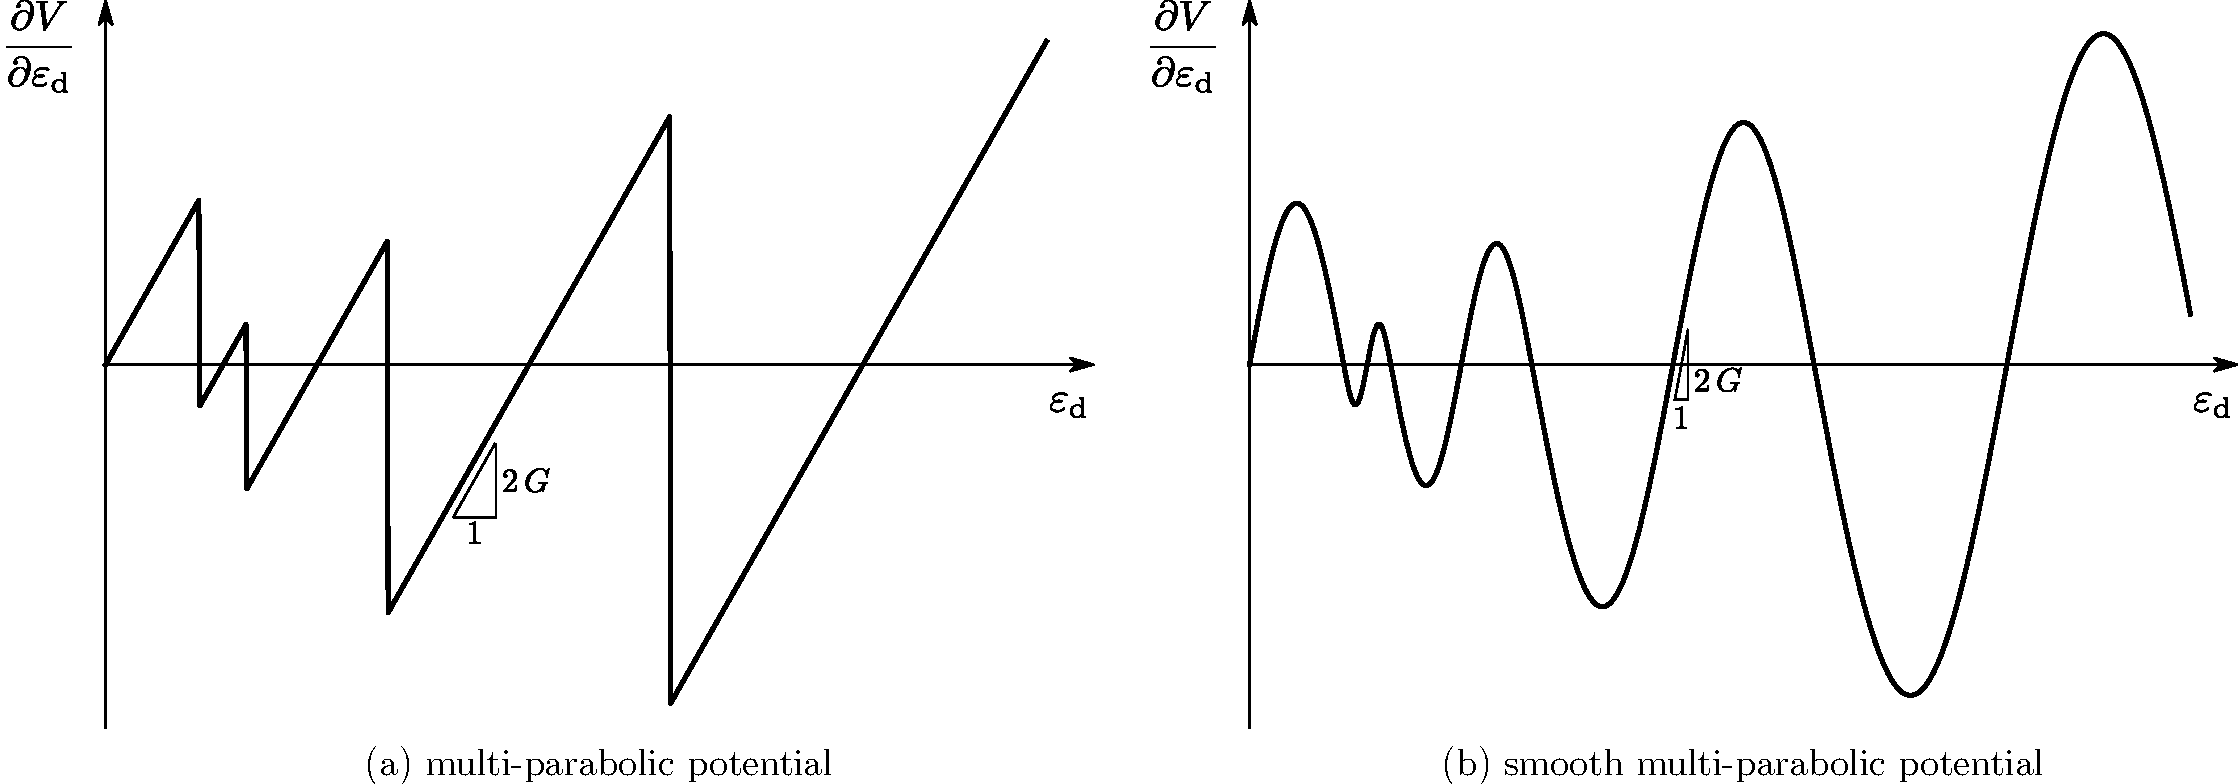
\includegraphics[width=1.\textwidth]{figures/potential_dV-plas}
    \caption{Derivative of the shear strain energy $V$.}
    \label{fig:dV:plas}
\end{figure}

\section{Specialized model -- planar shear}

\subsection{Motivation}

The model as proposed above treats all shear modes equally
(because $V$ is function of $\varepsilon_\mathrm{d}$).
Consequently it is isotropic.
There are, however, cases for which an anisotropic model is more realistic.
Below a model is proposed in which the plasticity can only occur along a specific plane.
Before that, the claim of isotropy is further motivated in two dimensions.
In that case the strain tensor has three independent modes,
illustrated in \cref{fig:strain-modes:2d}.

\begin{figure}[htp]
    \centering
    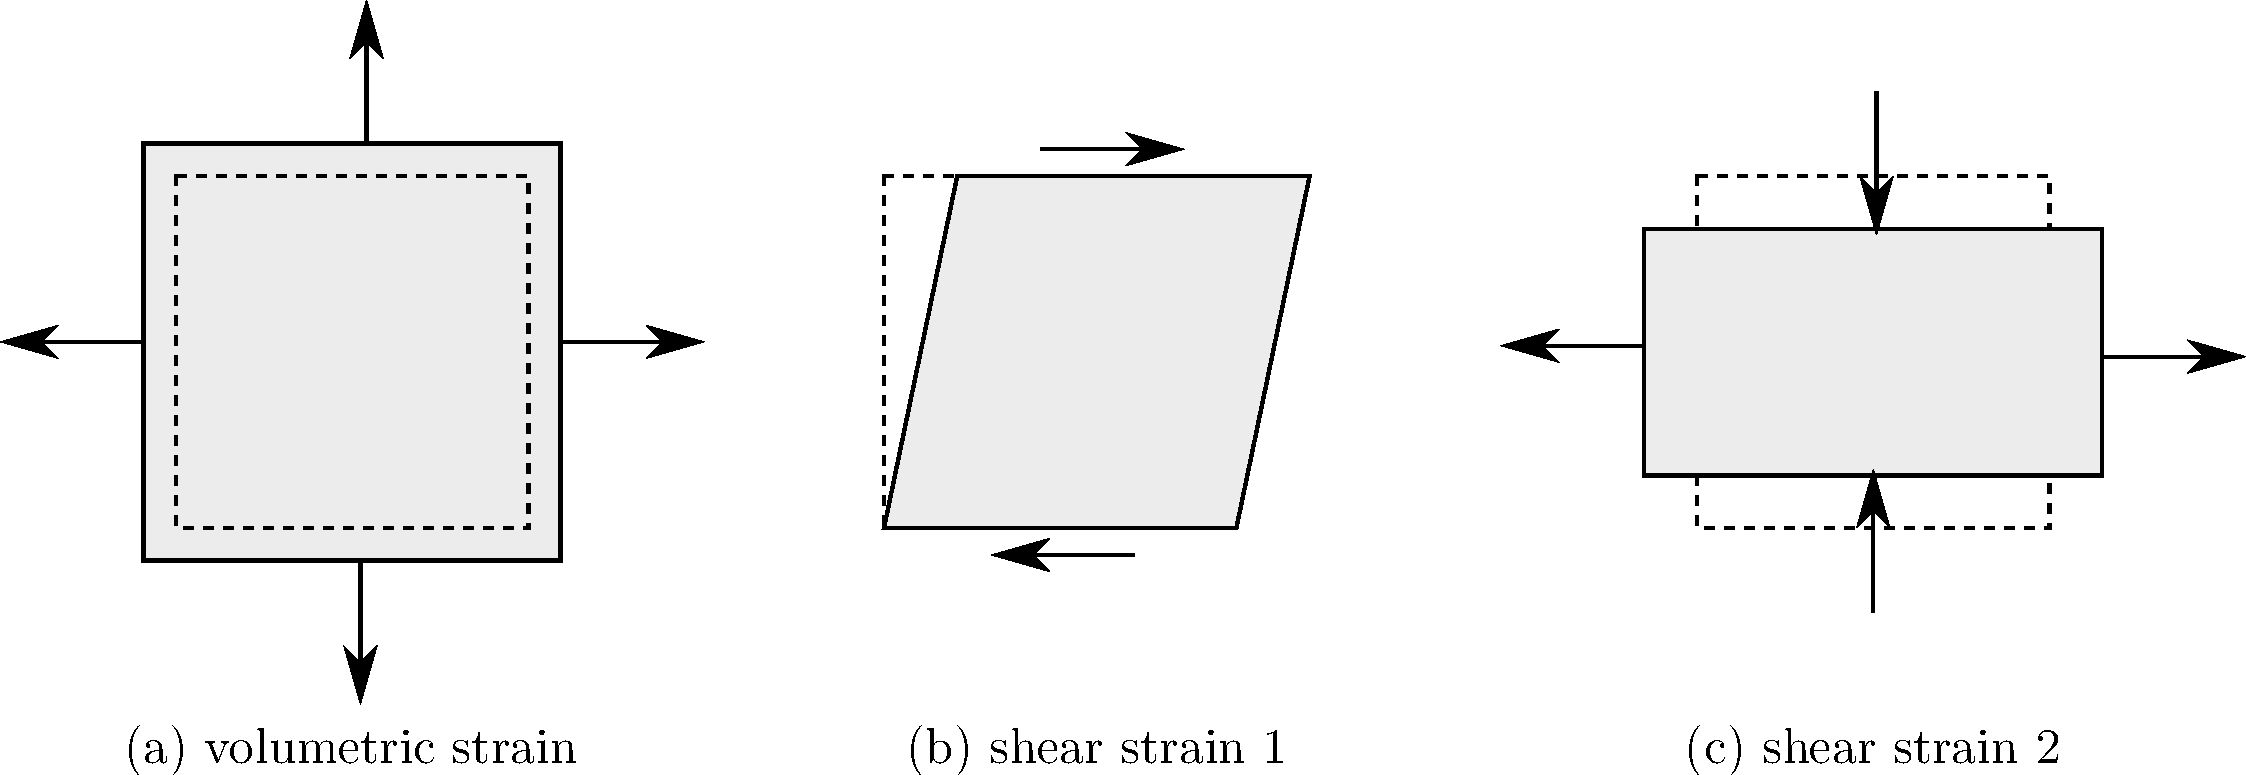
\includegraphics[width=.7\textwidth]{figures/strain-modes_2d}
    \caption{The three independent modes described by a 2-d stain tensor $\T{\varepsilon}$.}
    \label{fig:strain-modes:2d}
\end{figure}

The first shear mode, in \cref{fig:strain-modes:2d}(b),
corresponds to a strain tensor of the following structure
\begin{equation}
    \label{eq:strain-modes:basic}
    \underline{\underline{\varepsilon}}
    =
    \begin{bmatrix}
        0 & \gamma \\
        \gamma & 0
    \end{bmatrix}
\end{equation}
The second shear mode, in \cref{fig:strain-modes:2d}(c),
corresponds to the same shear deformation rotated by $-\pi/4$.
It is therefore of the structure
\begin{equation}
    \underline{\underline{\varepsilon}}
    =
    \begin{bmatrix}
        \gamma & 0 \\
         0 & -\gamma
    \end{bmatrix}
\end{equation}

In terms of the equivalent shear strain, both modes result in $\varepsilon_\mathrm{d} = |\gamma|$.
This is further illustrated by rotating the strain tensor
from \cref{eq:strain-modes:basic} by an angle $\theta$:
\begin{equation}
    \underline{\underline{\varepsilon}}^\prime
    =
    \underline{\underline{R}} \,
    \underline{\underline{\varepsilon}} \,
    \underline{\underline{R}}^T
\end{equation}
where the rotation matrix depends on the rotation angle $\theta$ as follows
\begin{equation}
    \underline{\underline{R}}
    =
    \begin{bmatrix}
        \cos \theta & - \sin \theta \\
        \sin \theta & \cos \theta
    \end{bmatrix}
\end{equation}
Trivially $\varepsilon_\mathrm{d} = | \gamma |$, independent of $\theta$ --
as plotted in \cref{fig:shear-modes:epseq} in black.
The contributions of the two shear modes are examined by examining $\varepsilon^\prime_{xy}$,
representative of the first shear mode in \cref{fig:strain-modes:2d}(b),
and $\varepsilon^\prime_{xx}$,
representative of the second shear mode in \cref{fig:strain-modes:2d}(c).
These contributions are plotted in \cref{fig:shear-modes:epseq} respectively in green and red.
Indeed, the contributions of the two shear modes vary with $\theta$,
while $\varepsilon_\mathrm{d}$ it is oblivious to this rotation.

\begin{figure}[htp]
    \centering
    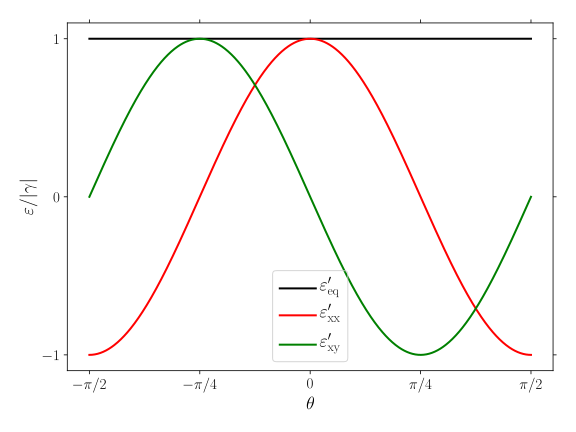
\includegraphics[width=.5\textwidth]{figures/strain-modes_2d_epseq}
    \caption{
        Comparison between the equivalent shear strain $\varepsilon_\mathrm{d}^\prime$
        the strain along the $x$-plane,
        $\varepsilon_\mathrm{s}^\prime
        = \varepsilon_{xy}^\prime
        = \vec{e}_x \cdot \T{\varepsilon}^\prime \cdot \vec{e}_y$,
        and the strain perpendicular to it,
        $\varepsilon_\mathrm{n}^\prime
        = \varepsilon_{xx}^\prime
        = \vec{e}_x \cdot \T{\varepsilon}^\prime \cdot \vec{e}_x$.
        For a 2-d simple shear strain tensor that is rotated by $\theta$ with respect
        to the $x$-axis,
        and normal $\vec{n} = \vec{e}_y$.}
    \label{fig:shear-modes:epseq}
\end{figure}

\subsection{Model}

In this model, the plasticity will be localised on a plane with normal $\vec{n}$
(which has unit length $||\, \vec{n} \,|| \equiv 1$), see \cref{fig:strain-vector-planar}.
To do so, the strain deviator $\T{\varepsilon}_\mathrm{d}$ is decomposed in two parts,
the strain along the plastic (`weak') plane $\T{\varepsilon}_\mathrm{s}$,
and the remaining strain $\T{\varepsilon}_\mathrm{n}$.
I.e.
\begin{equation}
    \label{eq:planar:strain:decomposition}
    \T{\varepsilon}_\mathrm{d} = \T{\varepsilon}_\mathrm{s} + \T{\varepsilon}_\mathrm{n}
\end{equation}
To compute the former, planar strain tensor $\T{\varepsilon}_\mathrm{s}$,
first the direction of the deviatoric stain tensor projected on the plane is determined as
\begin{equation}
    \vec{s}_\mathrm{n} =
    \frac{
        \T{\varepsilon}_\mathrm{d} \cdot \vec{n}
    }
    {
        ||\, \T{\varepsilon}_\mathrm{d} \cdot \vec{n} \,||
    }
\end{equation}
The strain direction along the plane is now found by projecting $\vec{s}_\mathrm{n}$ on it:
\begin{equation}
    \vec{s} =
    \frac{
        \vec{s}_\mathrm{n} - ( \vec{s}_\mathrm{n} \cdot \vec{n} )\, \vec{n}
    }
    {
        ||\, \vec{s}_\mathrm{n} - ( \vec{s}_\mathrm{n} \cdot \vec{n} )\, \vec{n} \,||
    }
\end{equation}
The amount of strain in this direction is finally found to be
\begin{equation}
    \varepsilon_\mathrm{s} = \vec{s} \cdot \T{\varepsilon}_\mathrm{d} \cdot \vec{n}
\end{equation}
Note that $\varepsilon_\mathrm{s}$ is by definition non-negative,
i.e.\ it is oblivious to rotations about $\vec{n}$.

The planar deviatoric strain tensor can now be constructed:
\begin{equation}
    \T{\varepsilon}_\mathrm{s} = \varepsilon_\mathrm{s}
    \big(
        \vec{s} \otimes \vec{n} + \vec{n} \otimes \vec{s}
    \big)
\end{equation}
From this it is obvious that $\varepsilon_\mathrm{s}$ is
the equivalent shear strain of this tensor, i.e.
\begin{equation}
    \varepsilon_\mathrm{s}
    \equiv
    \sqrt{ \tfrac{1}{2} \T{\varepsilon}_\mathrm{s} : \T{\varepsilon}_\mathrm{s} }
\end{equation}
(To show this one has to use that $\vec{n} \cdot \vec{n} \equiv 1$ and
$\vec{s} \cdot \vec{s} \equiv 1$ while $\vec{n} \cdot \vec{s} \equiv 0$).

\begin{figure}[htp]
    \centering
    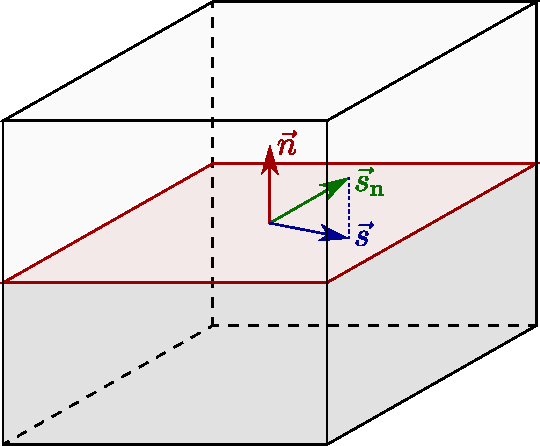
\includegraphics[width=.35\textwidth]{figures/strain-vector-planar}
    \caption{
        Strain along a plane defined by its normal $\vec{n}$:
        the strain vector $\vec{s}_\mathrm{n}$ and its planar projection $\vec{s}$.}
    \label{fig:strain-vector-planar}
\end{figure}

The remaining strain can now be trivially obtained from \cref{eq:planar:strain:decomposition} as
\begin{equation}
    \T{\varepsilon}_\mathrm{n} = \T{\varepsilon}_\mathrm{d} - \T{\varepsilon}_\mathrm{s}
\end{equation}
Its equivalent shear strain reads
\begin{equation}
    \varepsilon_\mathrm{n}
    = \sqrt{\tfrac{1}{2} \T{\varepsilon}_\mathrm{n} : \T{\varepsilon}_\mathrm{n}}
\end{equation}

For plasticity to occur only along the `weak' plane, the shear strain energy is further
decomposed in a planar part $V_\mathrm{s}$ that will be plastic,
and a non-planar part $V_\mathrm{n}$ that will be elastic:
\begin{equation}
    V
    =
    V_\mathrm{s} ( \varepsilon_\mathrm{s} )
    +
    V_\mathrm{n} ( \varepsilon_\mathrm{n} )
\end{equation}
Based on the definitions of the elastic and plastic potentials the
following expression for the stress is obtained
\begin{equation}
    \T{\sigma} ( \T{\varepsilon} )
    =
    K \, \varepsilon_\mathrm{m} \, \T{I}
    +
    G \, \T{\varepsilon}_\mathrm{n}
    +
    G \,
    \left[ \frac{\Delta \varepsilon_\mathrm{y}^{(i)}}{\pi} \right]
    \sin \left(
        \frac{ \pi }{ \Delta \varepsilon_\mathrm{y}^{(i)} }
        \Big[\, \varepsilon_\mathrm{s} - \varepsilon_\mathrm{min}^{(i)} \,\Big]
    \right)
    \frac{\T{\varepsilon}_\mathrm{s}}{\varepsilon_\mathrm{s}}
    \quad
    \mathrm{for}
    \;
    \varepsilon_\mathrm{y}^{(i)} \leq \varepsilon_\mathrm{s} < \varepsilon_\mathrm{y}^{(i+1)}
\end{equation}

\appendix

\vfill\newpage

\section{Tensors and tensor products}
\label{sec:nomenclature:tensor}

\begin{itemize}

    \item Second order tensor
    \begin{equation}
        \T{A} = A_{ij} \vec{e}_i \vec{e}_j
    \end{equation}

    \item Dyadic tensor product
    \begin{align}
        \T{C} &= \vec{a} \otimes \vec{b} \\
        C_{ij} &= a_{i} \, b_{j}
    \end{align}

    \item Double tensor contraction
    \begin{align}
        C
        &= \T{A} : \T{B} = \mathrm{tr} \left( \T{A} \cdot \T{B} \right) \\
        &= A_{ij} \, B_{ji}
    \end{align}

\end{itemize}

\section{Unit tensors}
\label{sec:nomenclature:unit}

\begin{itemize}

    \item Second order unit tensor
    \begin{equation}
        \T{I} = \delta_{ij} \vec{e}_i \vec{e}_j
    \end{equation}
    It is easy to show that it has the property that
    \begin{equation}
        \T{I} : \T{A} = \mathrm{tr} ( \bm{A} )
    \end{equation}

    \item Fourth order unit tensor:
    \begin{equation}
        \TT{I} : \T{A} \equiv \T{A}
    \end{equation}
    i.e.
    \begin{equation}
        \delta_{il} \delta_{jk} A_{lk} = A_{ij}
    \end{equation}
    hence
    \begin{equation}
        \TT{I} = \delta_{il} \delta_{jk} \vec{e}_i \vec{e}_j \vec{e}_k \vec{e}_l
    \end{equation}

    \item Deviatoric projection
    \begin{equation}
        \TT{I}_\mathrm{d} : \T{A} \equiv \T{A} - \tfrac{1}{d} \mathrm{tr} ( \bm{A} ) \T{I}
    \end{equation}
    hence
    \begin{equation}
        \TT{I}_\mathrm{d} = \TT{I} - \tfrac{1}{d} \T{I} \otimes \T{I}
        = \left( \delta_{il} \delta_{jk} - \tfrac{1}{d} \delta_{ij} \delta_{kl} \right)
        \vec{e}_i \vec{e}_j \vec{e}_k \vec{e}_l
    \end{equation}

\end{itemize}

\section{Strain measures}
\label{sec:nomenclature::strain}

\begin{itemize}

    \item Volumetric strain (in $d$ dimensions)
    \begin{equation}
        \varepsilon_\mathrm{m}
        = \tfrac{1}{d} \, \mathrm{tr} ( \T{\varepsilon} )
        = \tfrac{1}{d} \, \T{\varepsilon} : \T{I}
    \end{equation}

    \item Strain deviator
    \begin{equation}
        \T{\varepsilon}_\mathrm{d}
        = \T{\varepsilon} - \tfrac{1}{d} \, \mathrm{tr} ( \T{\varepsilon} ) \, \T{I}
        = \T{\varepsilon} - \varepsilon_\mathrm{m} \, \T{I}
        = \TT{I}_\mathrm{d} : \T{\varepsilon}
    \end{equation}

    \item Equivalent shear strain
    \begin{equation}
        \varepsilon_\mathrm{d}
        = \; \sqrt{
          \tfrac{1}{2} \, \T{\varepsilon}_\mathrm{d} : \T{\varepsilon}_\mathrm{d}
        }
    \end{equation}

\end{itemize}

\section{Stress measures}
\label{sec:nomenclature::stress}

\begin{itemize}

    \item Hydrostatic stress (in $d$ dimensions)

    \begin{equation}
        \sigma_\mathrm{m}
        = \tfrac{1}{d} \, \mathrm{tr} ( \T{\sigma} )
        = \tfrac{1}{d} \, \T{\sigma} : \T{I}
    \end{equation}

    \item Stress deviator

    \begin{equation}
        \T{\sigma}_\mathrm{d}
        = \T{\sigma} - \tfrac{1}{d} \, \mathrm{tr} ( \T{\sigma} ) \, \T{I}
        = \T{\sigma} - \sigma_\mathrm{m} \, \T{I}
        = \TT{I}_\mathrm{d} : \T{\sigma}
    \end{equation}

    \item Equivalent shear stress
    \begin{equation}
        \sigma_\mathrm{d} = \sqrt{ 2 \, \T{\sigma}_\mathrm{d} : \T{\sigma}_\mathrm{d} }
    \end{equation}

\end{itemize}

\section{Derivatives}
\label{sec:nomenclature:derivatives}

\begin{itemize}

    \item Trace of the strain
    \begin{equation}
        \frac{ \partial \, \mathrm{tr} ( \T{\varepsilon} ) }{ \partial \T{\varepsilon} }
        =
        \frac{ \partial }{ \partial \T{\varepsilon} } \left( \T{\varepsilon} : \T{I} \right)
        =
        \frac{ \partial \T{\varepsilon} }{ \partial \T{\varepsilon} } : \T{I}
        =
        \TT{I} : \T{I}
        =
        \T{I}
    \end{equation}

    \item Strain deviator
    \begin{equation}
        \frac{\partial \T{\varepsilon}_\mathrm{d}}{\partial \T{\varepsilon}}
        =
        \frac{\partial}{\partial \T{\varepsilon}}
        \left( \T{\varepsilon} - \tfrac{1}{d} \mathrm{tr} ( \T{\varepsilon} ) \T{I} \right)
        =
        \TT{I} - \tfrac{1}{d} \T{I} \otimes \T{I}
        =
        \TT{I}_\mathrm{d}
    \end{equation}

    \item Equivalent shear strain
    \begin{equation}
        \frac{ \partial \varepsilon_\mathrm{d} }{ \partial \T{\varepsilon} }
        =
        \frac{\partial}{\partial \T{\varepsilon}}
        \sqrt{\tfrac{1}{2}\, \T{\varepsilon}_\mathrm{d} : \T{\varepsilon}_\mathrm{d}}
        =
        \frac{1}{2 \varepsilon_\mathrm{d}}
        \frac{1}{2}
        \left[\, \frac{\partial \T{\varepsilon}_\mathrm{d}}{\partial \T{\varepsilon}}
        : \T{\varepsilon}_\mathrm{d} + \T{\varepsilon}_\mathrm{d}
        : \frac{\partial \T{\varepsilon}_\mathrm{d}}{\partial \T{\varepsilon}} \,\right]
        =
        \frac{1}{4 \varepsilon_\mathrm{d}}
        \big[\, \TT{I}_\mathrm{d} : \T{\varepsilon}_\mathrm{d}
        + \T{\varepsilon}_\mathrm{d} : \TT{I}_\mathrm{d} \,\big]
        =
        \frac{1}{2}
        \frac{\T{\varepsilon}_\mathrm{d}}{\varepsilon_\mathrm{d}}
        \equiv
        \tfrac{1}{2}
        \T{N}_d
    \end{equation}

\end{itemize}

\section{Conversion to common parameters for linear elasticity}

The parameters are confronted to their common definitions
(denoted here with a tilde) for linear elasticity in $d = 3$:

\begin{itemize}

    \item Bulk modulus
    \begin{equation}
        \kappa = K / 3
    \end{equation}

    \item Shear modulus
    \begin{equation}
        \mu = G / 2
    \end{equation}

\end{itemize}
This results in a stress response
\begin{equation}
    \T{\sigma} ( \T{\varepsilon} )
    =
    \kappa \, \mathrm{tr} ( \T{\varepsilon} ) \T{I}
    +
    2 \mu \left[ \T{\varepsilon} - \tfrac{1}{3} \mathrm{tr} ( \T{\varepsilon} ) \T{I} \right]
    =
    \kappa \, \mathrm{tr} ( \T{\varepsilon} ) \T{I}
    +
    2 \mu \, \T{\varepsilon}_\mathrm{d}
\end{equation}

\bibliography{library}

\end{document}
